\externaldocument{content/registration}
\chapter[Automatic Viewpoint Selection for Interactive Motor Feedback Using PCA]{Automatic Viewpoint Selection for Interactive Motor Feedback Using Principal Component Analysis\label{chap:viewpoint}}
In modern society, skill training is crucial across various areas, including recreational sports, physical therapy, and professional environments. Enhancing the learning process through interactive technology is becoming increasingly important. Specifically, in motor skill training supported by \acrshort{mr} technologies, interactive visual corrective feedback has become particularly significant, as demonstrated in \autoref{chap:visualCueSurvey}. This feedback is designed to support individuals to perform specific body movements correctly, thereby reducing the need for constant supervision by professionals. Superimposed avatars, in various types, represent a particular prevalent feedback method. Proper execution of movements is vital in physiotherapy and physical exercise to achieve the desired benefits and prevent injuries. Additionally, the repetitive and controlled nature of movements in physiotherapy and strength training allows for precise feedback provision and the identification of common errors.

Despite their importance, current methods for viewpoint selection in human motion and action feedback do not adequately consider visual cues. Furthermore, many existing techniques are computationally intensive and unsuitable for real-time application. In contrast, this chapter identifies key factors for optimal viewpoint selection for superimposed avatars used for motor feedback and propose an algorithm for this purpose using \emph{\acrshort{pca}}.

\section{Related Work \label{sec:relView}}
As demonstrated by Bouwmans et al.~\cite{bouwmans2018arpca}, robust \acrshort{pca} has numerous applications in the field of visual computing. For instance, Skaro et al.~\cite{skaro2021knac} introduced a \acrshort{pca}-based method to reduce errors common in motion tracking with markers.

Several studies have explored approaches to viewpoint selection for human actions or movements. For example, Rudoy et al.~\cite{rudoy2011vsh} developed a method to generate a three-dimensional volume from several successive frames to select the best physical camera for television broadcasts and similar applications. Whereas Kiciroglu et al.~\cite{kiciroglu2020amc} proposed an algorithm predicting pose estimation accuracy. As a result, a drone was navigated to the calculated optimal view point. Shi et al.~\cite{shi2012ksb} introduced an algorithm to determine the best viewpoint using \emph{Kinematics Significance Based Saliency}, which rotates figures and objects to show their most protuding features.

\begin{figure}[t!b]
	\centering
	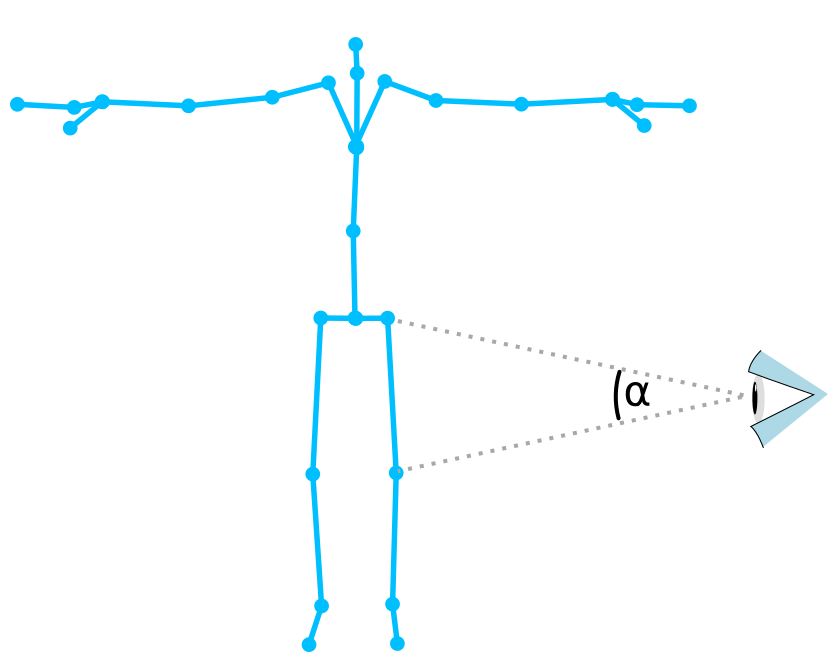
\includegraphics[width=0.6\linewidth]{pictures/skeleton_E_occ.png}
	\caption[Measure for the self-occlusion of the skeleton by Ishara et al.~\cite{ishara2015mra}.]{Measure for the self-occlusion of the skeleton by Ishara et al.~\cite{ishara2015mra}: \acrlong{jmo}.}
	\label{fig:jmo}
\end{figure}

Wang et al.~\cite{wang2019asw} utilized information theory and deep reinforcement learning to select a single viewpoint for action sequences. Simiarly, Choi et al.~\cite{choi2012rav} extracted key frames from motion data to create a sequence of stick figures representing the initial motion data.

Ishara et al.~\cite{ishara2015mra} calculated the optimal camera position for robot navigation using a camera mounted on top of the robot. Their approach involves calculating the so-called \emph{\acrfull{jmo}}, which considers the angle \(\alpha\) between two joints and the viewpoint, as shown in \autoref{fig:jmo}. The angles \(\alpha_{nm}\) between joints \(n\) and \(m\) are summed and normalized, where \(n,m \in N\) and \(n \neq m\), with \(N\) representing the number of joints. This approach results in \(\frac{N!}{2(N-2)!}\) calculations of \(\alpha\)~\cite{charalambides2002enumerative} and could therefore be computationally expensive. 

Kwon et al.~\cite{kwon2020ocp} proposed a method that results in a weighted sum of three metrics: \emph{normalized limb length}, \emph{normalized area of a 2-D bounding box}, and \emph{normalized visible area of a 3-D bounding box}. In addition, they also presented an algorithm that avoids recalculating weights for each frame by summing the three metrics without weights. However, their algorithm, designed for static poses, requires recalculation for each frame in videos. Despite these methods automatically selecting camera positions for human poses, they are insufficient for visual feedback, as the skeleton can occlude the feedback, making it difficult to perceive, as analyzed by Nundy et al.~\cite{nundy2000wam} and discussed in \autoref{sec:considerations}.

The approaches by Ishara et al.~\cite{ishara2015mra} and Kwon et al.~\cite{kwon2020ocp} were compared to our method in a subsequent user study, as they were the only methods applicable to human figures with feedback. For more details, see \autoref{sec:evaluation}.

\acrshort{pca} is commonly used to reduce dimensionality in data sets for machine learning~\cite{sorzano2014sdr}. The principal components represent the main independent directions in which data points spread. For spatial data, three independent directions are involved. The first two principal components represent the main spread directions, while the third component provides a good viewing direction, perpendicular to the first two. This is equivalent to reducing the dimensionality from three to two, as the rendered image of 3D objects is displayed in two dimensions. Assa et al.~\cite{assa2008moh} used this method to calculate camera paths. However, their use case differs significantly from ours, as they compute camera paths that involve camera cuts, which we avoid due to the short duration of exercise repetitions where cuts can be disorienting. Additionally, the work of Assa et al. is action-based, while ours is feedback-based, requiring additional measures to ensure feedback visibility. Lastly, their approach is not real-time capable, being computationally intensive and requiring the entire motion sequence for computation.

\section{Methodology \label{sec:view:methodology}}
\begin{figure*}[b!]
	\centering
	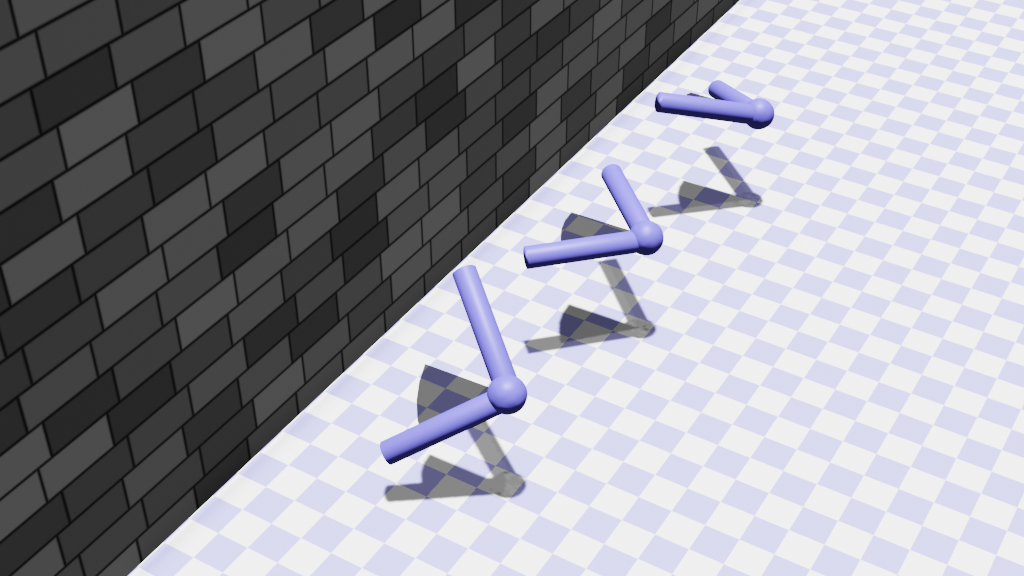
\includegraphics[width=0.49\linewidth]{pictures/projection_feedback}\hfill
	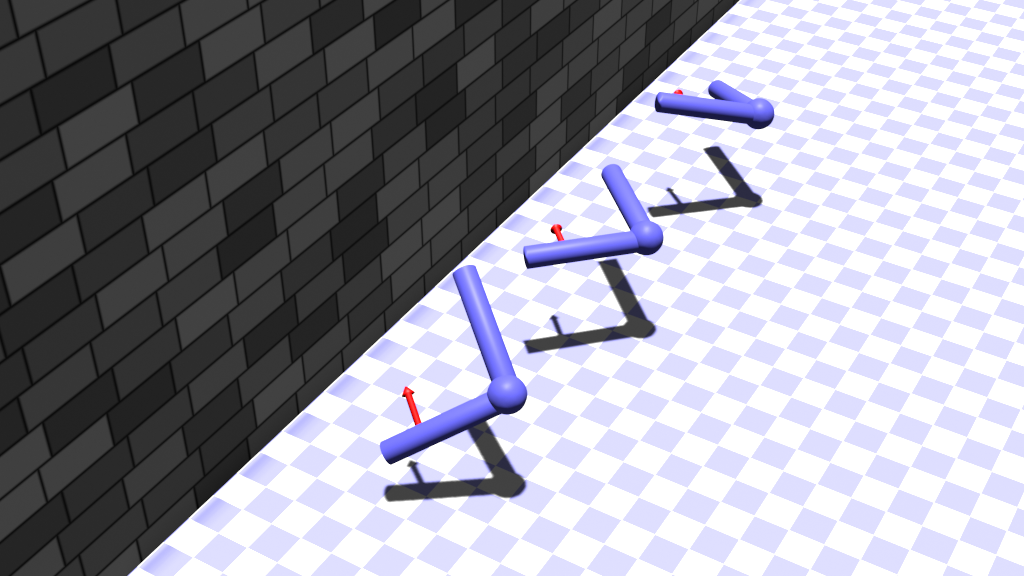
\includegraphics[width=0.49\linewidth]{pictures/projection_feedback_arrow}
	\caption[Feedback for the same angle viewed from different perspectives.]{Feedback for the same angle viewed from different perspectives. Two feedback cues: circular sector (left) and arrow (right). From left to right: Perfectly visible, visible, and hardly visible feedback. The shadows demonstrate that viewpoint affects not only the perception of the geometry but also of the feedback.}
	\label{fig:projection_feedback}
\end{figure*}
To facilitate a user-friendly and intuitive viewpoint selection, several things have to be considered. We will discuss these in detail in \autoref{sec:considerations}. With the foundational registration methods discussed in \autoref{chap:registration}, it is possible to calculate an optimized viewpoint, as presented in \autoref{sec:methViewCalc}.

\subsection{Perspective Considerations \label{sec:considerations}}
In the literature, concrete general rules for generating good perspectives are lacking. However, based on user preferences and logical argumentation several criteria and hints can be extracted to determine what facilitates a good viewpoint.

\begin{figure}[bt]
	\centering
	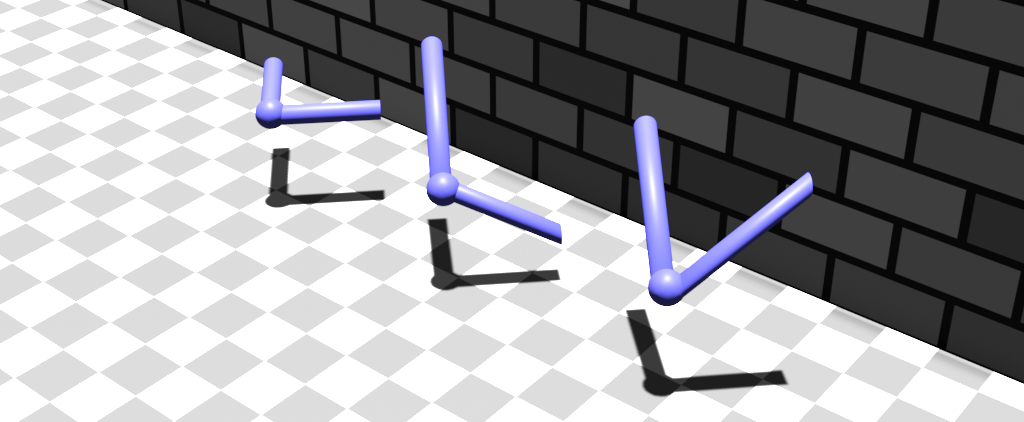
\includegraphics[width=\linewidth]{pictures/projection_normal.png}
	\caption[Illustrating the importance of viewpoint selection.]{Illustrating the importance of viewpoint selection: Three \emph{different} joint angles produce \emph{identical} shadows when projected onto the ground, implying they appear identical from an overhead perspective. Inspired by Nundy et al.~\cite{nundy2000wam}.}
	\label{fig:projection_normal}
\end{figure}

Polonsky et al.~\cite{polonsky2005wii} identified seven measurable view descriptors but concluded that determining a universally good view of an object is challenging. None of the view descriptors alone provides a general measure of viewpoint quality. However, some clues are available for treating specific objects. For instance, Zusne~\cite{zusne1970vpf} empirically demonstrated that humans prefer a frontal view of objects with eyes and a face.

When looking at motor feedback, in particular superimposed avatars, the positions of the joints and the angles between limbs are particularly critical for understanding movements. However, as previously analyzed by Nundy et al.~\cite{nundy2000wam}, angle perception is highly perspective-dependent. This is especially true in computer-rendered perspectives due to screen projection distortions, as shown in \autoref{fig:projection_normal} and \autoref{fig:projection_feedback}. While stereoscopic viewing (e.g., in the real-world or via \acrshort{hmd}) helps depth perception and angle interpretation, monoscopic rendering does not offer the same possibilities. Additionally, occlusion can impede understanding of the human pose: In particular, when the avatar's limbs are rendered behind each other self-occlusion occurs. Similarly, visual feedback cues can be obscured by the avatar itself or by other cues, as depicted in \autoref{fig:projection_feedback} and \autoref{fig:skeletonFeedbackPerspective}.


\begin{figure}[t!h]
	\centering
	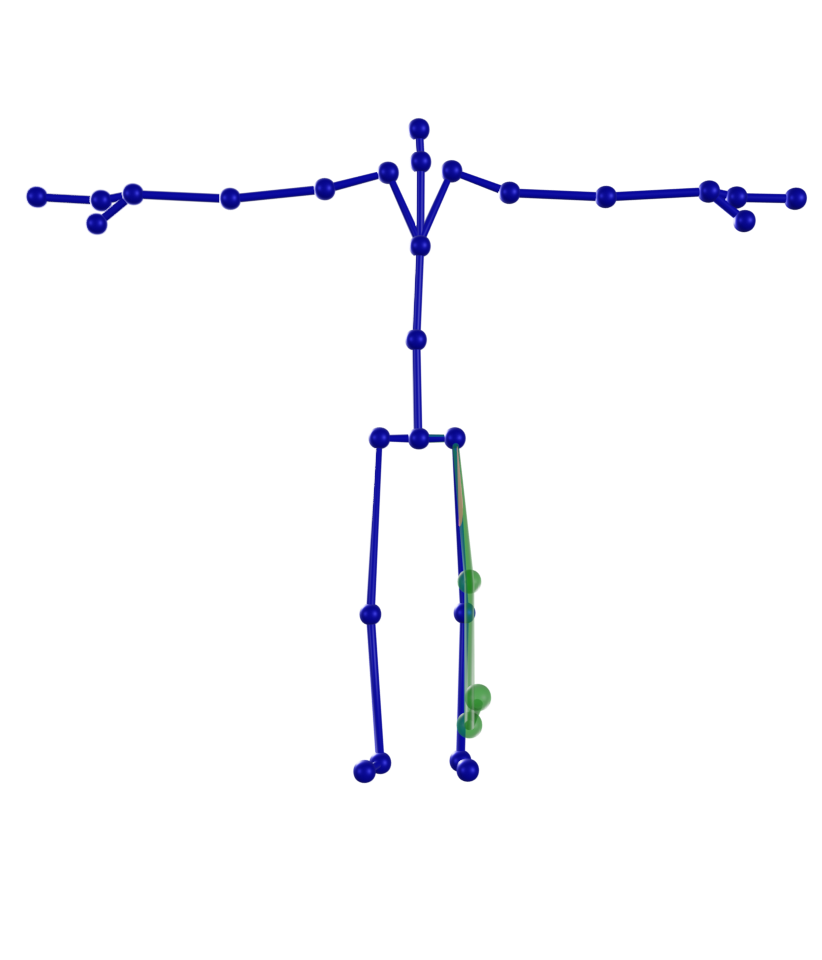
\includegraphics[width=0.49\linewidth]{pictures/feedbackFront.png}
	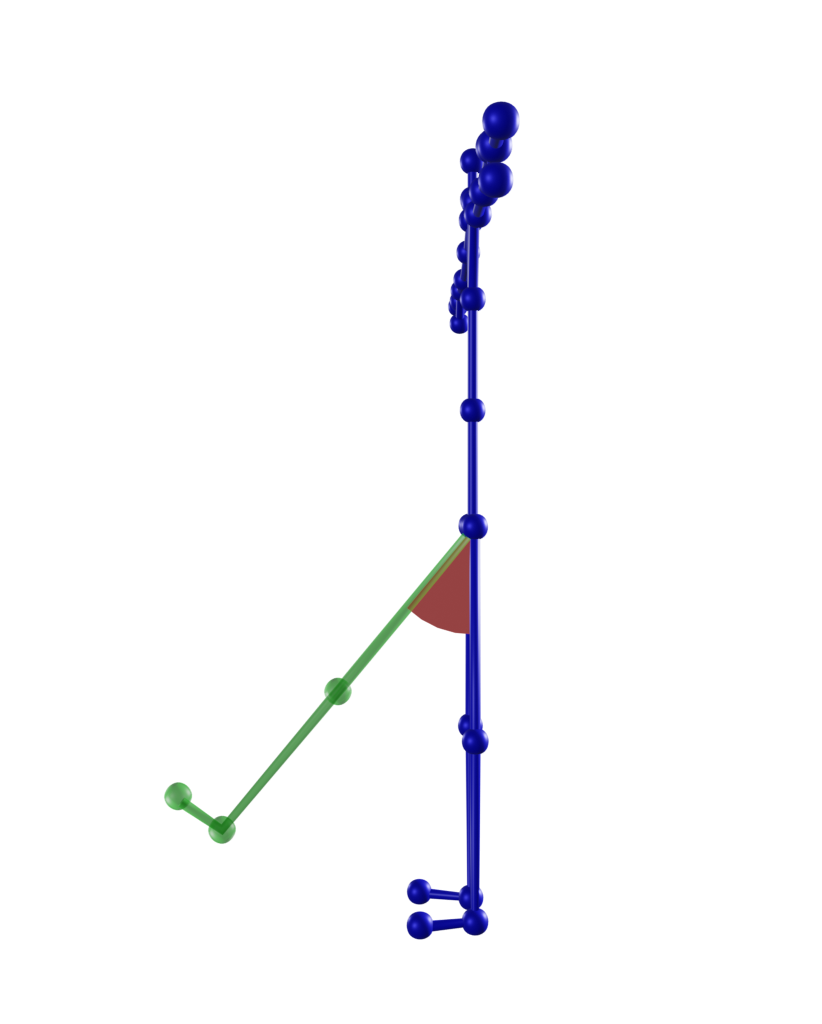
\includegraphics[width=0.49\linewidth]{pictures/feedbackSide.png}
	\caption[Skeleton of a human pose with feedback from two perspectives.]{Skeleton of a human pose with feedback from two perspectives. Two visual feedback cues are shown: A red angle sector and a superimposed avatar (here green skeleton). The feedback is hardly visible from the frontal perspective on the left.}
	\label{fig:skeletonFeedbackPerspective}
\end{figure}

Given the lack of a general description for a good view, we need to define the characteristics of a good viewpoint for our specific use case. In our context, we frequently use the metaphor of a virtual camera, common in rendering, to describe the viewpoint and viewing direction. Following Zusne's~\cite{zusne1970vpf} findings, we prefer an approximately frontal view of the human pose, meaning the virtual camera should be oriented towards the front of the pose rather than from behind. Additionally, the camera's up-vector should align with the world's up-vector to avoid viewer confusion, as this is the biologically typical perception for humans. Furthermore, we aim to minimize the occlusions of the avatars demonstrating the movement execution. Finally, in our use case, visual feedback is provided to correct movements or poses, and this feedback must be clearly visible. Therefore, feedback should not be occluded by the avatar or by itself and should be as perpendicular to the view direction as possible (compare \autoref{fig:skeletonFeedbackPerspective}).

When selecting perspectives for human motions and corresponding feedback, it is important to consider the dependencies of different body parts. Specifically, the limbs are hierarchically linked, meaning that moving the upper arm will cause the lower arm and hand to follow. Consequently, perspectives for such motions should ideally employ a \emph{hierarchical drill-down mechanism} to prioritize viewing along the hierarchy.

\subsection{Viewpoint Calculation \label{sec:methViewCalc}}

As presented in \autoref{sec:relView}, the existing literature does not yet provide an optimal viewpoint calculation for human motions with visual feedback suitable for skill learning. Most approaches are optimized for human actions, leading to the potential invisibility of feedback from an action-optimized viewpoint. In the following, we guide you through our computationally inexpensive method for calculating a viewpoint for human actions with feedback. \autoref{eq:viewpoint} shows the calculation of our view direction $\vec{v}_d$:

\begin{equation}
	\label{eq:viewpoint}
	\vec{v}_d = w \cdot \vec{v}_{S} + \sum_{n=1}^N (\Delta_n - \delta_0) \cdot \vec{v}_{Fn}
\end{equation}

Calculating $\vec{v}_d$ involves the following variables: \(w\) represents a weight to adjust the impact of the view between the whole skeleton and the feedback; \(\vec{v}_S\) is the viewpoint optimized for all joint coordinates (i.e., the actual skeleton); \(N\) represents the number of joints that exceed a given deviation threshold \(\delta_0\); \(\Delta_n\) is the deviation of a joint \(J_n\) from the intended target position; the variable \(\delta_0\) is a constant threshold of the deviation; and \(\vec{v}_{Fn}\) is the view direction optimized for the feedback corresponding to joint \(J_n\), i.e. the deviating of \(J_n\) and its corresponding joints, as seen in \autoref{fig:eigenvector}. We do not consider rotational deviations in the calculation, because they also inevitably cause deviations in distance (because of the \emph{hierarchical drill-down mechanism} mentioned in \autoref{sec:considerations}).

Some motion capture systems provide recorded spatial data as three-dimensional joint coordinates (see \autoref{sec:recording} for our data acquisition method). When we conduct \acrshort{pca} over such a point cloud of joint coordinates, the first two eigenvectors \(\vec{e}_{1S}\) and \(\vec{e}_{2S}\) represent the two main spatial spread directions. The third eigenvector \(\vec{e}_{3S} = \vec{v}_S\), perpendicular to the first two, consequently providing a well-suited view direction $\vec{v}$ for all joints, as explained in \autoref{sec:relReg}. In other words, the point cloud representing the whole skeleton is most spread out along the horizontal and vertical axes of the captured camera picture. Consequently, the view direction \(\vec{v}_S\) is optimal for comprehending motions and poses. This method is also presented in Assa et al.~\cite{assa2008moh}.

Because the view direction should be optimized for corrective feedback corresponding to the deviations of the exercises, we must consider the deviating joints. For this purpose, we locally apply the above-mentioned \acrshort{pca} viewpoint calculation. The \acrshort{pca} is conducted with the actual and target joint coordinates and the corresponding parent joint coordinates as seen in \autoref{fig:eigenvector} for joints \(J_n, n \in [1..N]\), with deviations \(\Delta_n\), that exceed the deviation threshold \(\delta_0\). Consequently, the resulting eigenvector \(\vec{e}_{3Fn} = \vec{v}_{Fn}\) is a suitable view direction for displaying joint \(J_n\), its parent, the corresponding optimal joint position, and its parent. This is illustrated in \autoref{fig:eigenvector}, where the considered joint \(J_n\) is shown in red, the optimal joint position in orange, and the corresponding parent joints are depicted in blue.

\begin{figure}[tb]
	\centering
	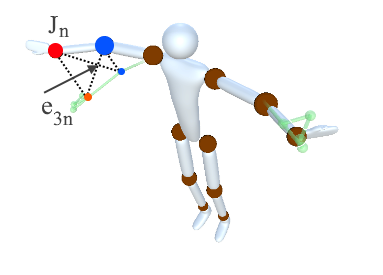
\includegraphics[width=0.5\linewidth]{pictures/eigenvector.png}
	\caption[PCA provides an optimal view direction for feedback.]{If Joint \(J_n\) (in red) deviates from the target position, a \acrshort{pca} is conducted including the corresponding target joint (in orange) and their parents (in blue). The eigenvector \(\vec{e}_{3n}\) then gives us an optimal view direction \(\vec{v}_{Fn}\) of the feedback for \(J_n\). The resulting view direction is orthogonal to the plane defined by the eigenvectors \(\vec{e}_{1n}\) and \(\vec{e}_{2n}\). This plane approximates the distribution of the considered joints and does not interpolate them.}
	\label{fig:eigenvector}
\end{figure}

In \autoref{eq:viewpoint}, the factor \(\Delta_n\) (minus the threshold \(\delta_0\)) of \(\vec{v}_{Fn}\) increases the influence of joints depending on their deviation. This automatically considers a hierarchical drill-down mechanism (see \autoref{sec:considerations}), since lower hierarchy joints (farther from the body center) usually have a higher absolute deviation, as they are impacted by the deviations of the higher hierarchy joints (closer to the body center), adhering to the intercept theorem. The subtraction of the threshold \(\delta_0\) ensures continuous camera movement, so that the impact of deviating joints continuously increases or sets in from zero. The sum of all \(\vec{v}_{Fn}\) represents a feedback-optimized view direction for all joints exceeding the deviation threshold. This could be seen as the calculation of the mean of all \(\vec{v}_{Fn}\) without the division. The division is discarded, as the length of the view direction vector is irrelevant.

The view direction optimized for the skeleton \(\vec{v}_S\) is weighted with the constant \(w\) to adjust optimization between the skeleton and feedback. Values of \(\delta_0 = 50\) and \(w = 3\delta_0 = 150\) showed the best empirical outcomes for our use case. This holds several implications:
\begin{itemize}
	\setlength{\itemsep}{-0.3cm}
	\item The eigenvectors resulting from the \acrshort{pca}, and therefore the view direction vectors, are normalized, i.e. they have a length of 1. In the virtual 3D space, we applied a scale of \(1\ unit = 1\ mm\). Consequently, the deviation threshold \(\delta_0\) corresponds to \(50\ mm\).
	\item To have the same impact as the skeleton-optimized view direction \(\vec{v}_S\), the feedback-optimized view direction \(\vec{v}_{Fn}\) of a single joint would need to have a deviation of 200 mm, consisting of a 50 mm minimal threshold plus 150 mm of weight.
	\item The deviations of several joints together can exceed 150 mm (plus threshold) to have the same impact on the resulting view direction as the skeleton as a whole.
	\item If multiple joints do not exceed the 50 mm minimal threshold, the skeleton has 100\% impact, thus the viewpoint is optimized for just the skeleton.
	\item Because we consider the absolute deviation (instead of relative to the parent), the deviations of lower hierarchy joints and their parent joints are dependent. This results in a hierarchical drill-down mechanism, as explained in \autoref{sec:considerations}, where the joints closer to the body center have a higher impact on the view direction.
\end{itemize}

To calculate the viewpoint for the virtual camera, we subtract the normalized view direction \(\vec{v}_d\) from the location of the focus point, which will be centered in the rendered frame (in our case, the joint representing the pelvis location, since it is a adequate representation of the body's center). The distance to the focused point (i.e. zoom) can be set by multiplying a constant. The digital distance corresponding to 2 m yielded the best results in our experiments, as all exercises were in frame at this distance. However, this highly depends on the settings (e.g., focal length) of the virtual camera chosen.


If \(\vec{e}\) is an eigenvector, \(c \cdot \vec{e}\) is also an eigenvector, for all \(c \neq 0\)~\cite{borisenko}. Consequently, \(-\vec{v}_d\), the flipped eigenvector of \(\vec{v}_d\), is also a viable view direction. Initially, we select the direction resulting in a more frontal view of the avatar, since this is the predominantly preferred view~\cite{zusne1970vpf}. For every subsequent frame, we select the direction (from \(\vec{v}_d\) and \(-\vec{v}_d\)) with a smaller angular difference from the previous frame's direction, ensuring smooth camera motion. This measure is applied to prevent the camera from switching between the view directions \(\vec{v}_d\) and \(-\vec{v}_d\).

Although the third eigenvector of the \acrshort{pca} follows a smooth path, the view direction (i.e. camera) tends to rotate around the avatar, contradicting Zusne's~\cite{zusne1970vpf} findings that a frontal view is commendable. To resolve this, we projected view angles from behind to the frontal plane, bypassing the predominantly small number of frames that feature a view from behind and showing a view from the side. Consequently, the projection affects the camera view only slightly and briefly.

Existing view selection approaches often focus on solving an optimization problem, iterating over a limited number of potential viewpoints, and choosing the one with the best score. This can result in a high number of costly iterations or erratic camera motion if the number of potential viewpoints is too small. Additionally, the best-scoring viewpoints in consecutive frames might be far from each other, resulting in inconsistent camera movements. Our method, however, provides continuous camera movement, as none of the mathematical operations in \autoref{eq:viewpoint} compromise consistency, and the \acrshort{pca} computations are conducted for continuously moving point clouds.

Empirically, no cases were encountered where a null vector arose from the calculations above. We also assessed stability regarding the \acrshort{pca}, as it is mathematically possible, that the camera view flips if the second and third eigenvectors have approximately the same length and deviate just slightly. In our experiments, this never occurred.

\section{Viewpoint Selection Evaluation \label{sec:evaluation}}
To verify the viewpoint selection method described in \autoref{sec:methViewCalc}, a user study was conducted. The necessary preliminaries, the study design, and the subsequent evaluation methods are found in the following.

\subsection{Participants}
For the user study, 39 individuals were recruited from an academic environment. These were predominantly computer science students between the ages of 20 and 30. More than half of the participants reported frequently exercising and considering movement-related aspects, giving ratings of four or higher on a five-point scale. This shows that the participants were somewhat acquainted with similar exercises and their execution. By comparison, much less physiotherapy clients were represented in the study. More than half of the participants reported the lowest frequency of receiving physiotherapy. Color vision deficiency did not affect our user study because the tasks required participants to recognize shapes rather than colors, as our focus was on perspective.

\subsection{Experimental Setup for Exercise Recording\label{sec:recording}}
The poses and motions found in this work were recorded using a Microsoft Azure Kinect 3D camera~\cite{kinect:documentation}. Its computer vision capabilities can provide spatial coordinates of several joints of the human body. Here, the term \emph{joint} is rather defined as biological landmarks than referring to the medical definition~\cite{kinect:documentation}.

The following conditions achieved optimal positioning of the subject in our case: The camera was mounted at about 140~cm with the help of a tripod. It was placed about 280~cm away from the subject. The height of the subject was about 190~cm. This setup allowed for stable tracking and captured all poses within the frame. According to our use case, the joints of the eyes, ears, and nose were discarded as we found that these were too imprecise and irrelevant for our use case. This left us with 26 joints. For further information on the visualization of avatars, see \autoref{sec:exercise}.

Subsequently, a diverse set of example exercises was developed including various exercise and deviation combinations. We then superimposed each of these exercises to the corresponding counterpart with deviation from the correct form (see \autoref{sec:sample}). The spatial registration was unambiguous, as the majority of joints were nearly identical. For further information regarding registration, covering more complex cases, see \autoref{sec:methReg}. The methods used to create an overlay of two exercises matching temporally exceed the scope of this chapter. Throughout the literature we often see \emph{Dynamic Time Warping} fulfilling that role (e.g., \cite{su2013pre}, \cite{anton2015pre}, and \cite{saenz2016kbv}).


\begin{figure*}[t!]
	\centering
	\subfloat[\centering Bench press]{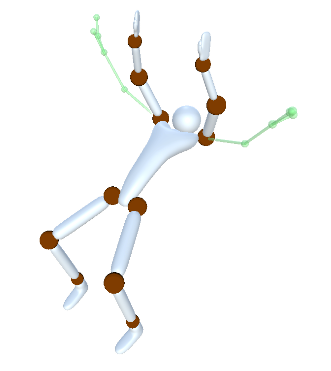
\includegraphics[width=.18\linewidth]{pictures/bench.png}\hfill}  
	\subfloat[\centering Curl A]{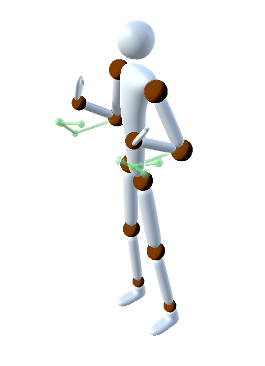
\includegraphics[width=.14\linewidth]{pictures/curlA.png}\hfill} 
	\subfloat[\centering Lateral raises]{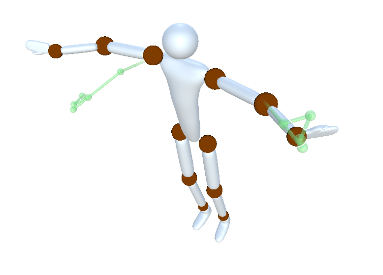
\includegraphics[width=.18\linewidth]{pictures/lateral.png}\hfill} 
	\subfloat[\centering Shoulder press]{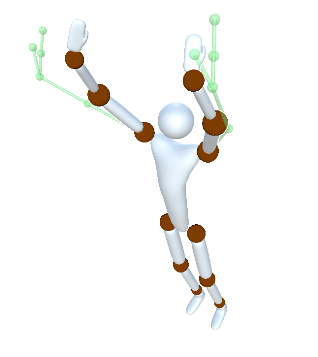
\includegraphics[width=.18\linewidth]{pictures/shoulder.png}\hfill} 
	\subfloat[\centering Bent-over\\row]{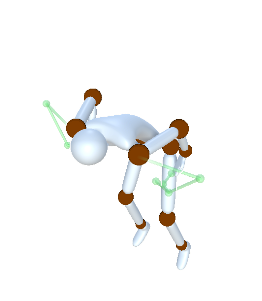
\includegraphics[width=.18\linewidth]{pictures/rows.png}\hfill}
	\subfloat[\centering Curl B]{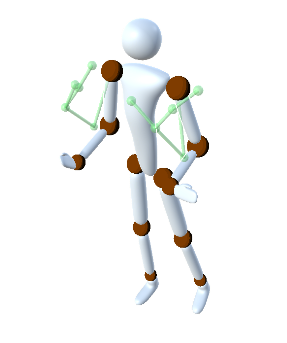
\includegraphics[width=.14\linewidth]{pictures/curlB.png}\hfill} 
	\caption{Sample exercises with deviations as described in \autoref{sec:sample}.}
	\label{fig:optimal:exercises}
\end{figure*}

\subsection{Exercise Visualization \label{sec:exercise}}
An abstract avatar was used to visualize the actual motion, and for the target motion, a skeleton is displayed as seen in \autoref{fig:optimal:exercises}. The visualization of the skeleton displayed in green corresponds to the joints recorded by the 3D camera~\cite{kinect:documentation} as mentioned in \autoref{sec:recording}. Two different avatar visualizations were used to help users distinguish the actual movement from the target movement. In addition, users with color vision deficiency are supported, as the differences between the avatars are distinguished by shape, not by color. The abstract avatar occludes itself and its background to a greater extent and visualizes fewer joint positions than the skeleton, as the fingertips and thumbs are integrated into the hand. Yet, for viewpoint optimization, all joints are considered in the calculations. The visualizations in this chapter are simply used for demonstrative purposes and are not the subject of our research. The focus of this work is the viewpoint selection. Therefore, visualization methods of the avatars and feedback play a subordinate role.

\subsection{Sample Exercises \label{sec:sample}}
To assess our method, as described in \autoref{sec:study}, and compare it with those described in existing literature, we selected four static poses to establish basic assumptions (see \autoref{sec:considerations}) and six dynamic exercises, each with specific deviations from the ideal form. The deviations were chosen to be common mistakes for the considered exercises. We aimed to select a wide variety of exercises and deviations to evaluate the methods exhaustively. As a result, the poses and exercises were selected in a way, that various movement and feedback directions are represented. For instance, during lateral raises, the arms are moved laterally away from the body, whereas in a biceps curl, the arms move in front of the body (see \autoref{fig:optimal:exercises}). We also included an exercise with different deviations (biceps curls A and B).

Selecting a viewpoint for videos can be considered as choosing a continuous viewpoint for each static pose in the individual frames. Hence, to verify the underlying assumptions of viewpoint quality (see \autoref{sec:considerations}), we chose four representative static poses: standing (standard anatomical position), squatting, bending down, and bench press. To learn more about how the user study was conducted, please refer to \autoref{sec:study}.

The following six exercises were chosen, including deviations (see \autoref{fig:optimal:exercises} for visualization of the exercises): bench press (deviation: Arms too wide), lateral raises (deviation: Arms asymmetrical), bent-over row (deviation: Elbows tucked in), shoulder press (deviation: Arms asymmetrical), biceps curl A (deviation: Repetition only executed halfway), and biceps curl B (deviation: Elbows do not stay stable). The exercises and their deviations were recorded at the same position, and performed by the same individual. Therefore, it was possible to use the absolute position as a registration method. However, the commendable methods described in \autoref{sec:methReg} would yield the same results, even when performed with different-sized individuals at varying positions.

\subsection{User Study Design \label{sec:study}}
The user study was divided into three tasks. The participants were presented with two interactive tasks and a set of structured questions. A detailed explanation of the tasks and questions is provided in the following.

\textbf{Viewpoint Selection:} We intended to confirm the underlying assumptions of user preferences for the views as explained in \autoref{sec:considerations}. For this purpose, users were asked to choose the best viewpoint for static poses. Visual feedback was not displayed during this task, as we wanted to verify the established assumptions. As viewpoint selection for videos selects a viewpoint for a static pose in each frame, this should give us insights into user preference for both cases and how our algorithm performs in comparison. Furthermore, it is unfeasible for users to select a camera path in real-time. Therefore, only with static poses user evaluation is even possible. As a result, it was possible to compare our method to the current literature (see \autoref{sec:relView}).

A skeleton-like avatar successively showed four static poses of exercises: Bench press, squat, bent-over row, and standing (for more information, see \autoref{sec:sample}). The users could adjust the view direction pose-wise by clicking and dragging the mouse. A skybox around the avatar supported orientation in virtual 3D. After confirming, the viewpoint was captured and stored for analysis.

\textbf{Viewpoint Comparison:} To evaluate the performance of our view selection algorithm, we randomly juxtaposed four looped videos of exercise repetitions with the corresponding correction feedback. The viewpoint in each video was selected by a different method. This way, six different exercises with deviations were successively shown, as explained in \autoref{sec:sample}.  

The different methods used for viewpoint selection are:
\begin{itemize}
	\setlength{\itemsep}{-0.3cm}
	\item Ishara et al.~\cite{ishara2015mra}, who selected the viewpoint by calculating the \emph{\acrshort{jmo}}, the biggest sum of angles between all joints and the potential viewpoint (see \autoref{fig:jmo}).
	\item The method of Kwon et al.~\cite{kwon2020ocp} involves the sum of displayed limb lengths, a 2D, and 3D bounding box. As their best resulting method is computationally intensive and not capable of real-time, we chose their second-best algorithm variant without weights.
	\item Our algorithm, as described in \autoref{sec:methViewCalc}.
	\item  To compare the methods to a neutral position, we included a viewpoint as it is used in \emph{isometric projection} (rotated 45° horizontally and 35.264° vertically).
\end{itemize}
For an in-detail explanation of the methods mentioned in this section, see \autoref{sec:relView}.

\textbf{Questionnaire:} Finally, the third task asked participants to provide more details about their prior experience with the topic and to share their opinions. The first four questions were answered using a Likert scale, while the last two were answered with free-text responses:

\begin{itemize}
	\setlength{\itemsep}{-0.3cm}
	\item How often do you exercise?
	\item How often are you involved in strength training?
	\item How often do you receive physiotherapy? 
	\item How often do you consider movements?
	\item What options would you have liked to see?
	\item What stood out to you?
\end{itemize} 

\subsection{Viewpoint Benchmark \label{sec:benchmark}}
The calculated viewpoints were evaluated using the benchmark presented by Dutagaci et al.~\cite{dutagaci2010bbv}. They provided a method to evaluate potential viewpoints and compare them to a selection of views chosen by users. The calculation of what Dutagaci et al. call the \acrfull{vse} can be found in \autoref{eq:vse}. The \acrshort{vse} represents a number between 0 and 1, where low values signify a high discrepancy between the viewpoints in question and the ones chosen by the users.

\begin{equation}
	\label{eq:vse}
	VSE = \frac{1}{M \cdot \pi \cdot r}\sum_{m=1}^{M} GD_{m}
\end{equation}

In \autoref{eq:vse}, \(GD_m\) represents the geodesic distance of the potential viewpoint to each user-chosen viewpoint \(m \in M\). The variable $M$ represents the total number of participants (i.e., the number of viewpoints to consider). The viewpoints are expected to be on a sphere (viewpoint sphere) around the focused object. The radius of said sphere (i.e. the distance of each viewpoint to the focused object) is represented by $r$. To visualize the user-selected viewpoints, the viewpoint vectors were projected on the median and transverse planes. Subsequently, we plotted the \acrshort{vse} by comparing each direction around the center as a potential viewpoint. As a result, the \emph{\acrshort{vse}} is displayed angle-wise in the median and frontal plane around the body using the Viridis colormap~\cite{viridis} in \autoref{fig:colorMaps}. Here, blue areas represent a low \acrshort{vse} and therefore, an overall low distance to the user-selected view directions. In contrast, view directions that were avoided by the participants are shown by yellow areas.

\begin{figure*}[t]
	\centering
	\subfloat[\centering Bench Press]{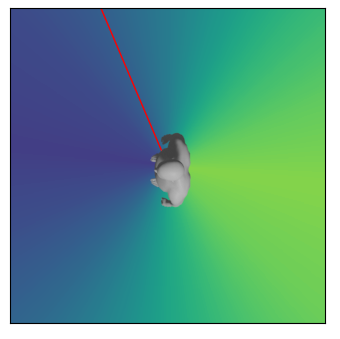
\includegraphics[width=0.24\linewidth]{pictures/transverseBench.png}}
	\subfloat[\centering Squat]{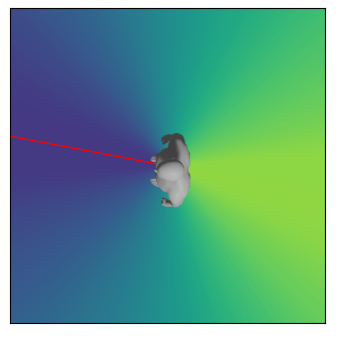
\includegraphics[width=0.24\linewidth]{pictures/transverseSquat.png}}
	\subfloat[\centering Bent-down]{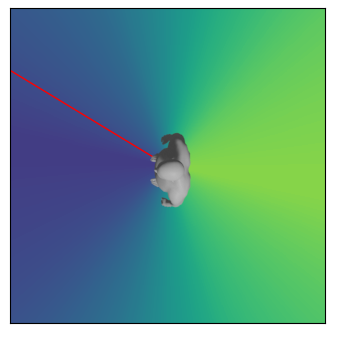
\includegraphics[width=0.24\linewidth]{pictures/transverseBend.png}}
	\subfloat[\centering Stand]{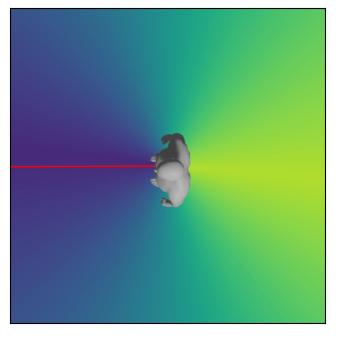
\includegraphics[width=0.24\linewidth]{pictures/transverseStand.png}}
\includegraphics[width=0.041\linewidth]{pictures/whitePixel.png}\\
	\subfloat[\centering Bench Press]{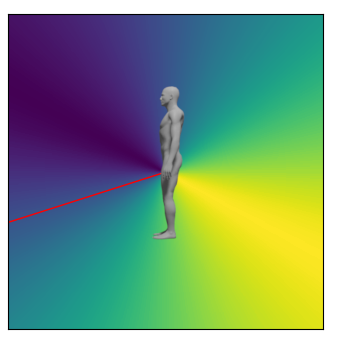
\includegraphics[width=0.24\linewidth]{pictures/medianBench.png}}
	\subfloat[\centering Squat]{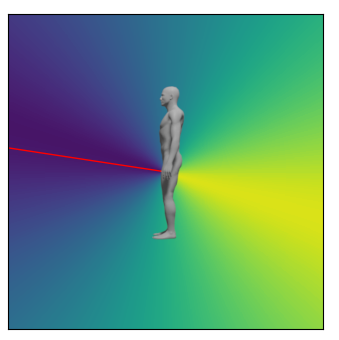
\includegraphics[width=0.24\linewidth]{pictures/medianSquat.png}}
	\subfloat[\centering Bent-down]{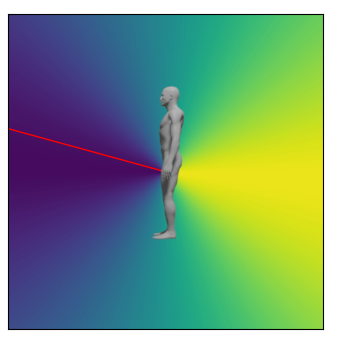
\includegraphics[width=0.24\linewidth]{pictures/medianBend.png}}
	\subfloat[\centering Stand]{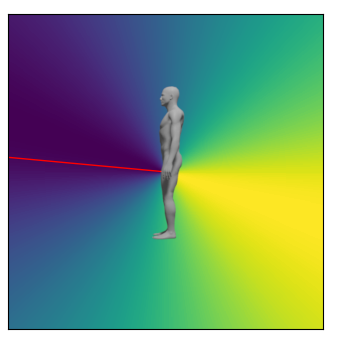
\includegraphics[width=0.24\linewidth]{pictures/medianStand.png}}    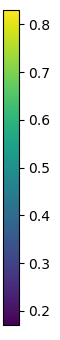
\includegraphics[width=0.041\linewidth]{pictures/scale.png}
	\caption[Comparison of our method to user selected view points.]{\acrfull{vse} for different viewing angles from the top (a-d) and side (e-h) using the benchmark of Dutagaci et al.~\cite{dutagaci2010bbv}. The red line represents the view direction selected by our method. The human figure only shows spatial orientation and does not represent the executed movements.}
	\label{fig:colorMaps}
\end{figure*}

\section{Results\label{results}}
In \autoref{sec:results:selection}, we will discuss the performance of each algorithm during the viewpoint selection task relative to the user-selected viewpoints, using the Dutagaci Benchmark as described in \autoref{sec:benchmark}. Subsequently, in \autoref{sec:results:analysis} the output of each method based on the exercise videos will be illustrated to give the reader an understanding of the results. Lastly, \autoref{sec:results:comparison} concludes the user study results of the viewpoint comparison. The results of the questionnaire are used in \autoref{sec:study} to specify the participants, and in \autoref{sec:insights}, the free-text answers are discussed.

\subsection{Viewpoint Selection \label{sec:results:selection}}
In \autoref{fig:colorMaps}, a low \acrshort{vse} is represented by blue areas. Therefore, viewpoints in these areas aligned well with the user selection. Yellow areas were chosen less. The red line represents the viewpoint chosen by our method for the static pose without movement. Looking at \autoref{fig:colorMaps}, we see that our method calculated viewpoints predominantly lying in the blue regions, i.e., in regions preferred by users. Similarly, it becomes apparent when analyzing the \acrshort{vse} mean over the four exercises, that, in comparison, our algorithm fits the selection of the users best with an average \acrshort{vse} of 0.3467. The static isometric-like view performed second best with an average \acrshort{vse} of 0.347 followed by \acrshort{jmo} with 0.4825 and the method of Kwon et al. with 0.5497.

\subsection{Method Analysis\label{sec:results:analysis}}
To interpret the comparison of methods in \autoref{sec:results:comparison}, it is essential to understand the viewpoints each method provides and how these viewpoints change over time.

\textbf{\acrshort{jmo}~\cite{ishara2015mra}:}
The \acrshort{jmo} algorithm predominantly produced an adequate overview of the human body. A major drawback was that, when applied to videos, the algorithm erratically switched between viewpoints that were significantly distant from each other. This can be perceived in \autoref{fig:jmoSequence}. Consequently, the feedback often was difficult to comprehend, as the algorithm was not designed to work with visual cues or videos. Additionally, several viewpoints were selected from below and behind, although participants preferred perspectives from the front and slightly above (see \autoref{sec:results:selection}).

\textbf{Kwon et al.~\cite{kwon2020ocp}:} 
As can be seen in \autoref{fig:kwonSequence}, the algorithm of Kwon et al. seemed to predominantly produce views from behind in our application. As elaborated in \autoref{sec:results:selection}, this is a view that is mostly avoided by users. Additionally, the algorithm sometimes selected views from below, similar to the \acrshort{jmo} algorithm mentioned earlier. The algorithm by Kwon et al. offered a much more stable perspective than \acrshort{jmo}. However, the feedback was often challenging to see.

\textbf{Ours:}
Our algorithm consistently transitioned between an optimal viewpoint for the neutral position and the contracted position with deviations, as illustrated in \autoref{fig:bicepsSequence}. When feedback was present, it was displayed clearly and with a perceivably emphasized. However, during some exercises, the rapid exercise execution caused a conflict between the neutral and the feedback-optimized viewpoint. This resulted in quick camera movements, which some users perceived as irritating.


\begin{figure*}[h!]
	\centering
	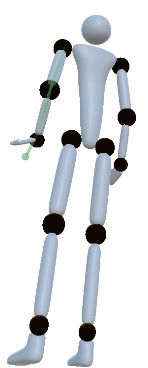
\includegraphics[width=0.11\linewidth]{pictures/kwonSequence1.png}\hfill
	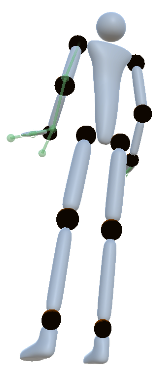
\includegraphics[width=0.12\linewidth]{pictures/kwonSequence2.png}\hfill
	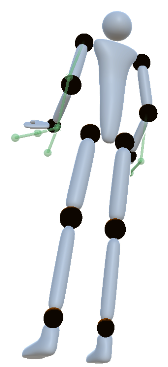
\includegraphics[width=0.12\linewidth]{pictures/kwonSequence3.png}\hfill
	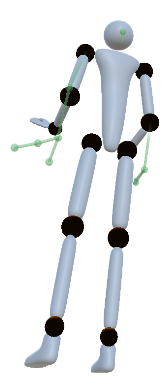
\includegraphics[width=0.12\linewidth]{pictures/kwonSequence4.png}\hfill
	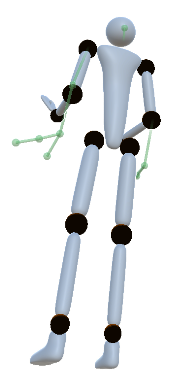
\includegraphics[width=0.12\linewidth]{pictures/kwonSequence5.png}\hfill
	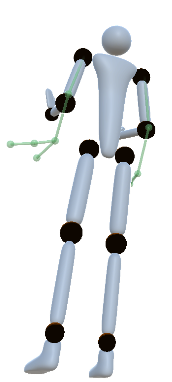
\includegraphics[width=0.12\linewidth]{pictures/kwonSequence6.png}\hfill
	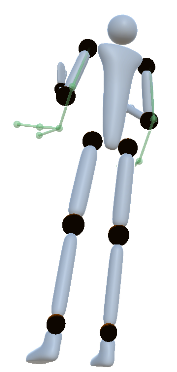
\includegraphics[width=0.12\linewidth]{pictures/kwonSequence7.png}\hfill
	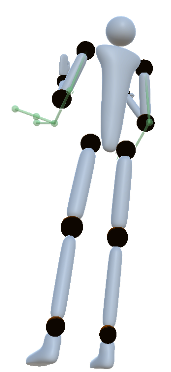
\includegraphics[width=0.115\linewidth]{pictures/kwonSequence8.png}\hfill
	\caption[Image sequence optimized by Kwon et al.~\cite{kwon2020ocp}.]{Image sequence, taken from a video of a biceps curl exercise with deviation. The viewpoint is optimized by the algorithm by Kwon et al.~\cite{kwon2020ocp}.}
	\label{fig:kwonSequence}
\end{figure*}

\begin{figure*}[h!]
	\centering
	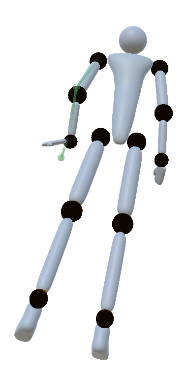
\includegraphics[width=0.11\linewidth]{pictures/jmoSequence1.png}\hfill
	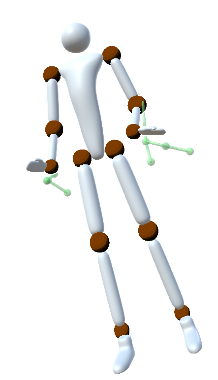
\includegraphics[width=0.12\linewidth]{pictures/jmoSequence2.png}\hfill
	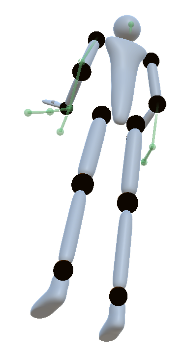
\includegraphics[width=0.12\linewidth]{pictures/jmoSequence3.png}\hfill
	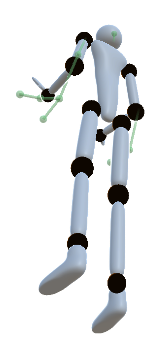
\includegraphics[width=0.10\linewidth]{pictures/jmoSequence4.png}\hfill
	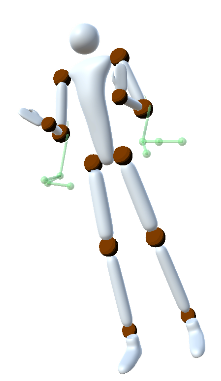
\includegraphics[width=0.12\linewidth]{pictures/jmoSequence5.png}\hfill
	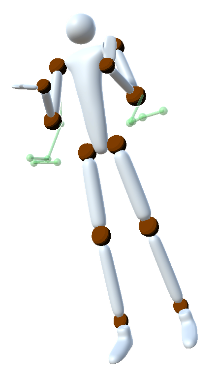
\includegraphics[width=0.12\linewidth]{pictures/jmoSequence6.png}\hfill
	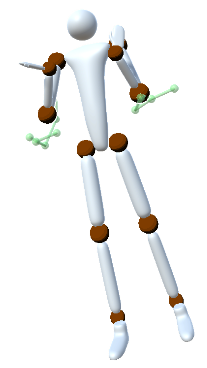
\includegraphics[width=0.12\linewidth]{pictures/jmoSequence7.png}\hfill
	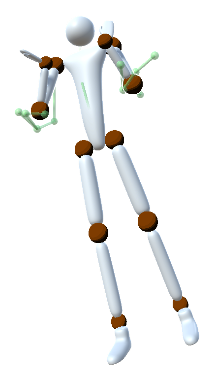
\includegraphics[width=0.12\linewidth]{pictures/jmoSequence8.png}\hfill
	\caption[Image sequence optimized by Ishara et al.~\cite{ishara2015mra}.]{Image sequence, taken from a video of a biceps curl exercise with deviation. The viewpoint is optimized by the \emph{\acrfull{jmo}} algorithm by Ishara et al.~\cite{ishara2015mra}.}
	\label{fig:jmoSequence}
\end{figure*}

\begin{figure*}[h!]
	\centering
	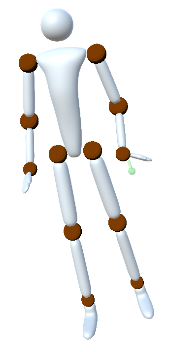
\includegraphics[width=0.115\linewidth]{pictures/bicepsSequence1.png}\hfill
	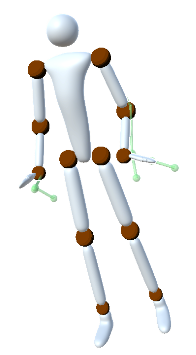
\includegraphics[width=0.13\linewidth]{pictures/bicepsSequence2.png}\hfill
	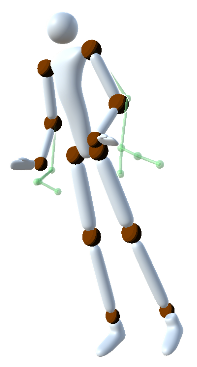
\includegraphics[width=0.125\linewidth]{pictures/bicepsSequence3.png}\hfill
	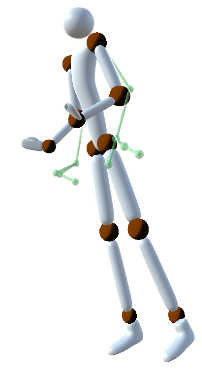
\includegraphics[width=0.125\linewidth]{pictures/bicepsSequence4.png}\hfill
	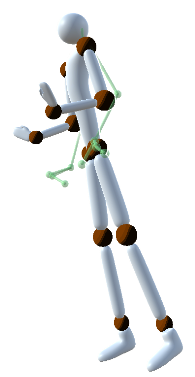
\includegraphics[width=0.12\linewidth]{pictures/bicepsSequence5.png}\hfill
	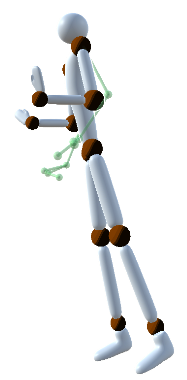
\includegraphics[width=0.115\linewidth]{pictures/bicepsSequence6.png}\hfill
	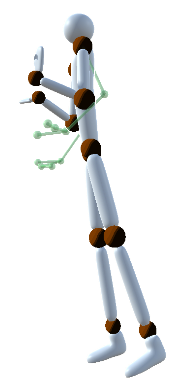
\includegraphics[width=0.11\linewidth]{pictures/bicepsSequence7.png}\hfill
	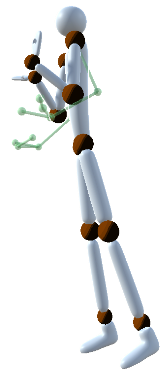
\includegraphics[width=0.11\linewidth]{pictures/bicepsSequence8.png}\hfill
	\caption[Image sequence optimized by our method.]{Image sequence, taken from a video of a biceps curl exercise with deviation. The viewpoint is optimized by our algorithm.}
	\label{fig:bicepsSequence}
\end{figure*}

\subsection{Viewpoint Comparison \label{sec:results:comparison}}

\autoref{tab:comparison} shows the user choice distribution of the viewpoint comparison. Our algorithm was most prevalent with 35.04~\% of votes, the isometric-like position was chosen second most with 32.48~\%, followed by Kwon et al.~\cite{kwon2020ocp} with 17.52~\% and lastly \acrshort{jmo}~\cite{ishara2015mra} with 14.96~\%.

Occasionally camera positions from behind were provided by the methods of Kwon et al.~\cite{kwon2020ocp} and Ishara et al.~\cite{ishara2015mra}. Additionally, they produced an unsteady camera movement, because they jumped between far-distant viewpoints and generally, had merely a limited amount of viewpoints available. In contrast, the static isometric-like viewpoint produced surprisingly good results, although it lacked an adaptation for movement or feedback. The primary advantage of the isometric-like viewpoint over the other methods was its stability. Our method provided an adequate view of the neutral positions of the exercises. Furthermore, it produced a continuous camera movement toward a feedback-oriented viewpoint with increasing deviation. However, the camera movement showing the bench press and bent-over row exercises was occasionally rapid.

\section{Insights and Discussion\label{sec:insights}}
Looking at \autoref{fig:colorMaps}, it becomes evident that the participants preferred a frontal view direction. This aligns with the statement made by Zusne~\cite{zusne1970vpf}, that humans desire frontal views (see \autoref{sec:considerations}), and verifies these requirements for our application. Additionally, it was observed that participants preferred a viewpoint from slightly above.

Our algorithm performs significantly less well for some specific exercises. This can be attributed to the consistently smooth, though occasionally rapid, camera movement. In particular, the camera moved rapidly during the bench press and bent-over row exercises. As stated in \autoref{sec:methViewCalc}, our algorithm generally prevents inconsistent camera movement, though rapid camera motions may still occasionally occur.

\begin{table}[b]
	\centering
	\caption[Results of user study evaluation view selection methods.]{\label{tab:comparison}Results of user study. Distribution of viewpoint selection methods chosen by the participants.}%
	\begin{tabular}{@{}l|llllll|l@{}}
		\toprule
		Method & \begin{sideways}Bench press\end{sideways} & \begin{sideways}Biceps curl A  \end{sideways} & \begin{sideways}Lateral raises\end{sideways} & \begin{sideways}Shoulder press\end{sideways} & \begin{sideways}Bent-over row\end{sideways} & \begin{sideways}Biceps curl B\end{sideways}  & \begin{tabular}{l}Total\\Percentage\end{tabular} \\
		\midrule
		Neutral  & 19 & 15 & 3 & 15 & 6 & 18 & 32.48 \% \\
		\acrshort{jmo} & 1 & 1  & 6  & 0 & 25 & 2 & 14.96 \% \\
		Kwon & 14 & 7  & 3  & 3 & 6 & 8 & 17.52 \% \\
		Ours  & 5 & 16 & 27  & 21 & 2 & 11 & \textbf{35.04 \%} \\
		\bottomrule
	\end{tabular}
\end{table}

The most prevalent statement made by the participants regarded camera movement consistency. Specifically, users were irritated by movements that were too rapid or erratic. This observation matches similar findings by Assa et al.~\cite{assa2008moh} concerning camera paths. Additionally, many participants indicated that having multiple camera perspectives would help them to understand the poses and feedback. This is especially interesting for future work and when applying suggested methods. Additionally, some users desired the option to select no method, as they felt none of the suggested perspectives were adequate. This implies that there are possible improvements to our algorithm and that human viewpoint preferences might need further assessment. Lastly, some users struggled to interpret poses without relation to the environment. Primarily, this concerned the bench press exercise, where a virtual bench might help users interpret the avatar posture. Therefore, incorporating the surrounding environment could facilitate understanding, especially for exercises involving equipment such as weights, benches, and pull-up bars. However, additionally rendered equipment could occlude the avatar or visual cues and therefore hinder the perception of the provided feedback.

The spatial registration (see \autoref{sec:methReg}) for our use case was trivial, since the superimposed exercises were recorded at the same position with the same individual. Other circumstances, like varying individuals or different registration methods can yield fundamentally different results in terms of feedback appearance. However, the view selection methods, as presented in \autoref{sec:methViewCalc}, would still select a valid viewpoint. Depending on what registration methods were chosen, the view selection could be skewed toward the feedback deviation. If other registration methods are chosen, it might be necessary to adapt the constants in the viewpoint selection calculation (in particular, $w$ and $\delta_0$ in \autoref{eq:viewpoint}) to retrieve the desired perspectives.

\section{Conclusion}
The chapter at hand provides novel insights on how to optimize the display of superimposed avatars including motion feedback. Current literature suggests, that the superimposition of avatars plays an increasingly important role. As an accessible and intuitive method of providing and receiving motor feedback, it is widespread in both \acrshort{mr} and traditional feedback technologies.

We introduce a new method for selecting viewpoints for motor feedback, such as superimposed avatars, among other options. Not only is this method computationally faster than the methods found in the literature, but evaluation in the context of a user study showed, that participants preferred our method over other approaches found in the literature.

Our viewpoint selection method combined with the registration methods found in \autoref{chap:registration} can adequately optimize the display of superimposed avatars. However, the individual methods provide value as well, as they can be utilized separately from each other.